An electron can be misidentified as a photon if the association of tracks or track seeds to the ECAL supercluster fails in the reconstruction step. 
The production of a single \PW\ boson decaying to an electron and a neutrino is a high-rate process, and it mimicks the photon plus \met\ signature if the electron is misidentified.

The rate at which this misidentification occurs is proportional to the inefficiency $1 - \epsilon_{\Pe}^{\text{track}}$ of the tracking, defined over the electrons passing the photon identification criteria described in Sec.~\ref{sec:pf_photons} except the electron veto. 
This partial identification is denoted as \Pe\Pgg\ ID in the following.  
If one assumes that the kinematic and other critical properties of the electron plus \met\ events are unaffected by the electron misidentification, it is possible to model the electron misidentification background by taking a proxy sample with well-identified electrons and scaling this sample by $R_{\Pe} = (1 - \epsilon_{\Pe}^{\text{track}}) / \epsilon_{\Pe}^{\text{track}}$.

The ``tag-and-probe'' method described in Section~\ref{sec:idsf} with appropriate changes is used to measure the efficiency corresponding to the factor $R_{\Pe}$ in data.

The first such change is that the sample is split into \Pe\Pgg\ and \Pe\Pe\ categories depending on whether the probe passes or fails the electron veto requirement. 
Probes in both categories must also pass the \Pe\Pgg\ ID.
Denoting the area of the peak in each cateogry  $N_{\Pe\Pgg}$ and $N_{\Pe\Pe}$, respectively, the ratio $N_{\Pe\Pgg} / N_{\Pe\Pe}$ is equal to $R_{\Pe}$ up to minor systematic corrections.

The second such change is in the background model used in the TP fits. 
The backgrounds to the \Pe\Pgg\ fit consist of processes with actual electron and photon in the final state, such as \PW\Pgg\ and \Zee\ with a hard radiation off one of the electrons.
Because of this, we scale the mass distrubition of the $\Pgm+\Pgg$ sample by the ratio of electron-probe to muon-probe events taken from MC to account for the different rates of FSR and bremsstrahlung between muons and electrons.
As an alternative template to assess the systematic effect introduced by the choice of the background template, the unscaled mass distribution is also tested.

%%% these fils have charged PF veto included, need to swap out
\begin{figure}[htbp]
  \begin{center}
    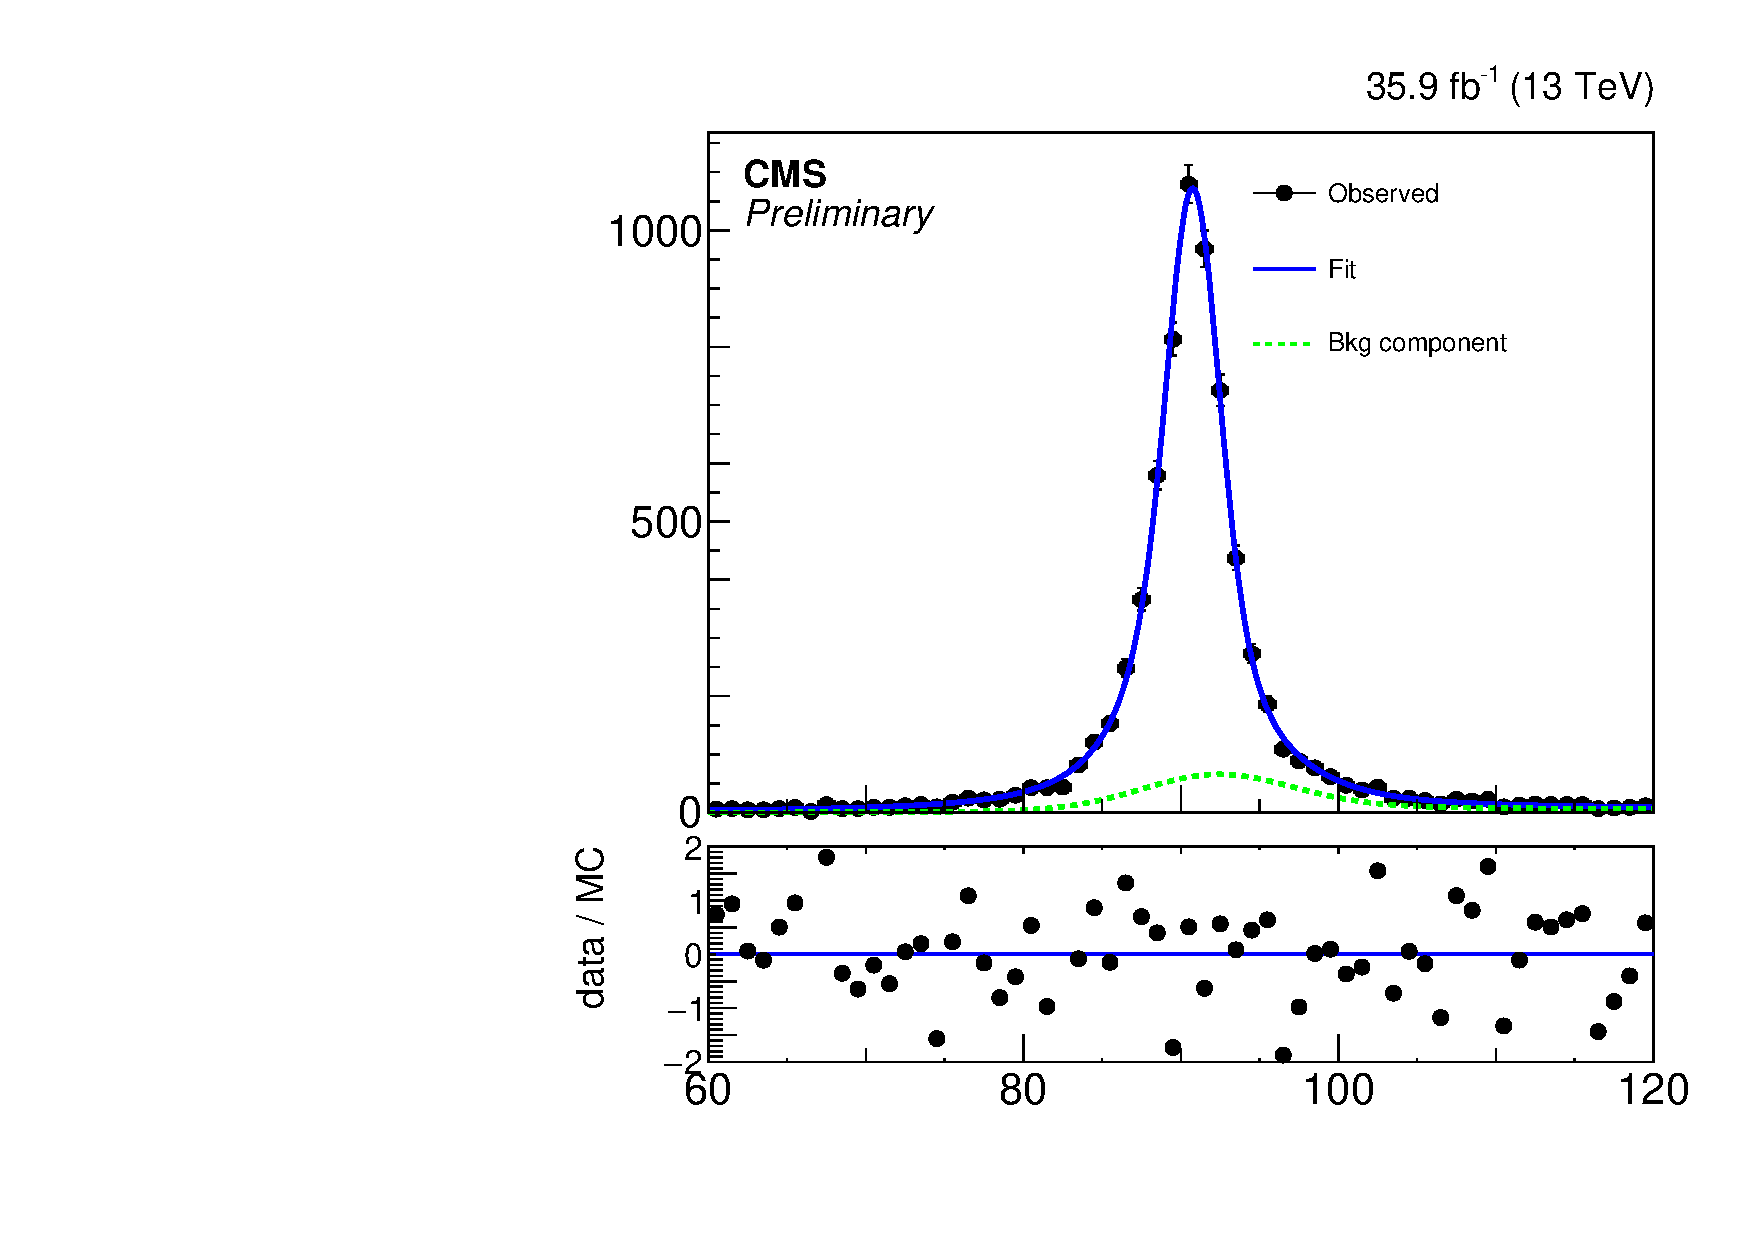
\includegraphics[width=0.47\textwidth]{Analysis/Figures/fit_data_ee_pt_175_200.pdf}
    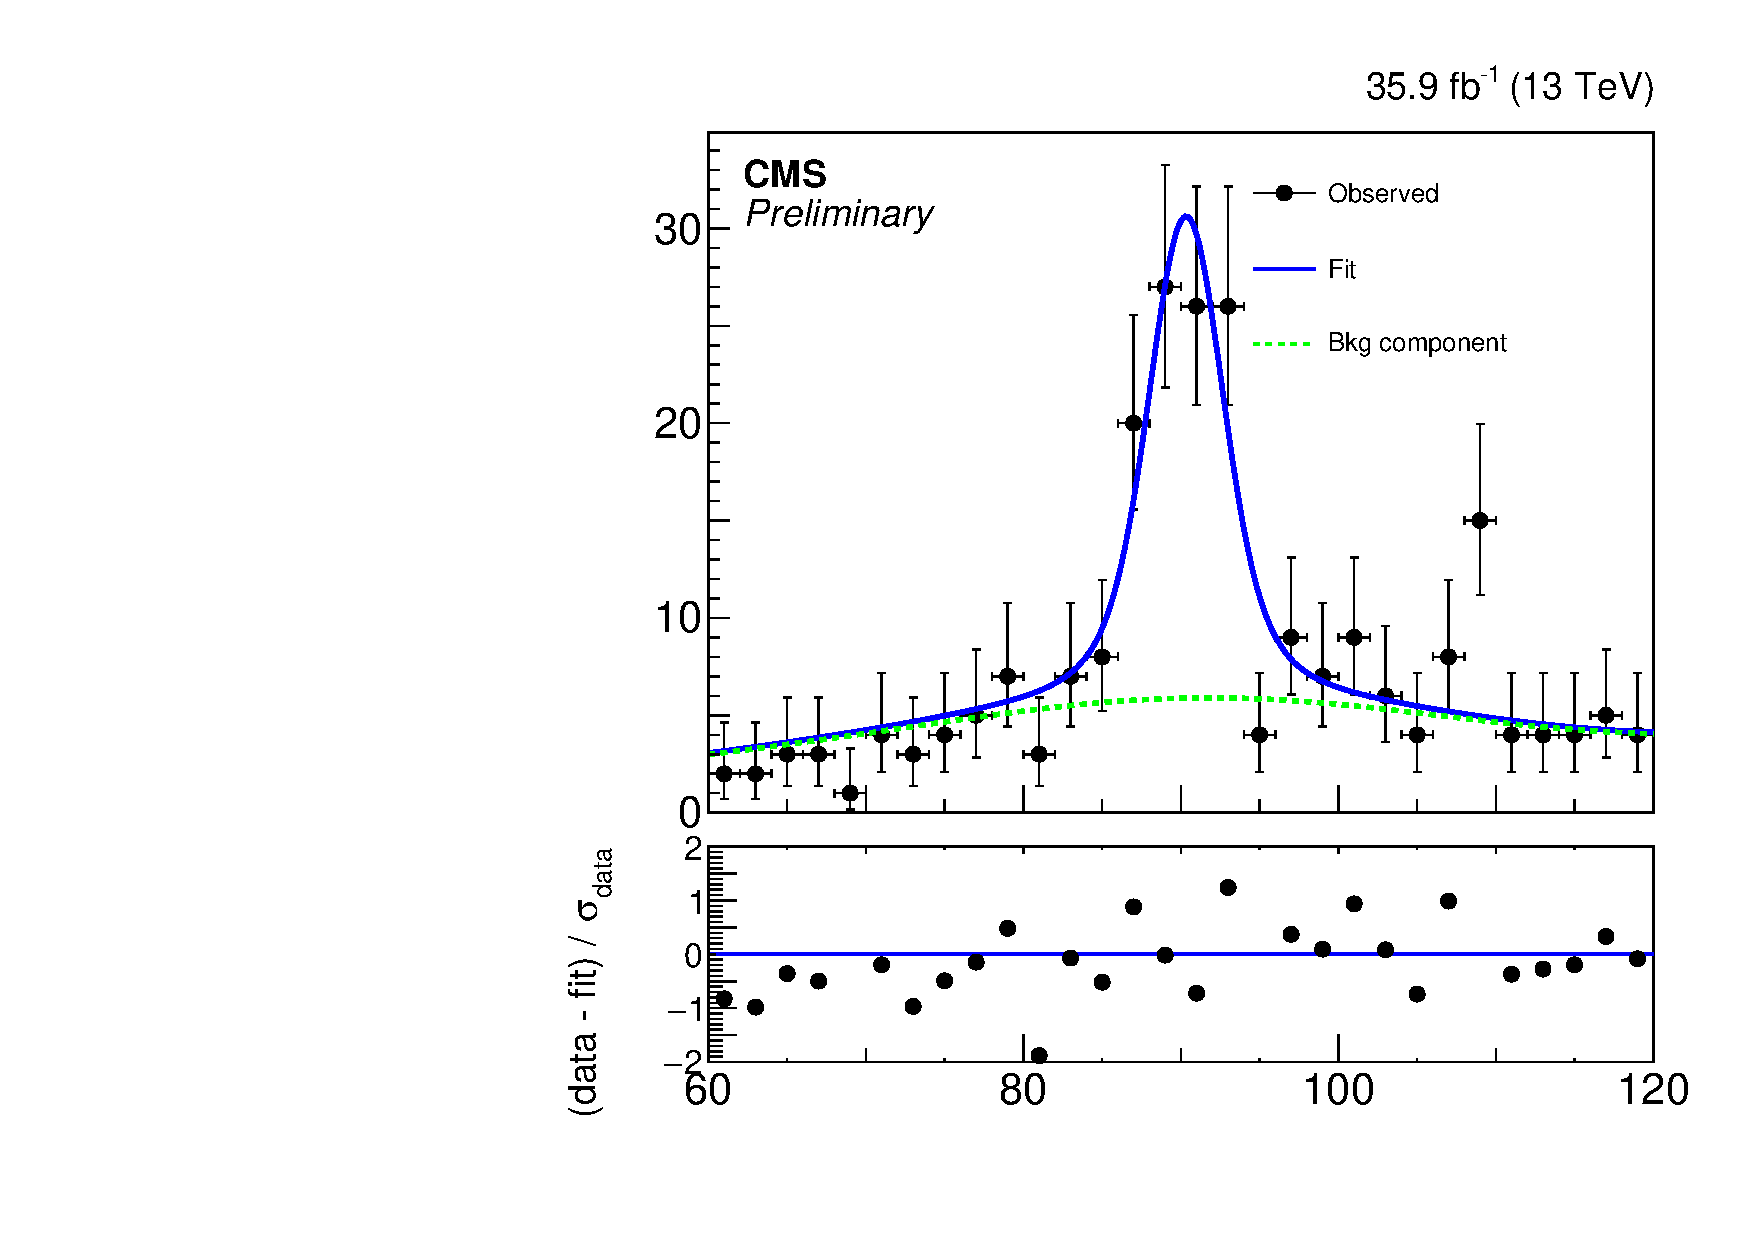
\includegraphics[width=0.47\textwidth]{Analysis/Figures/fit_data_eg_pt_175_200.pdf}
    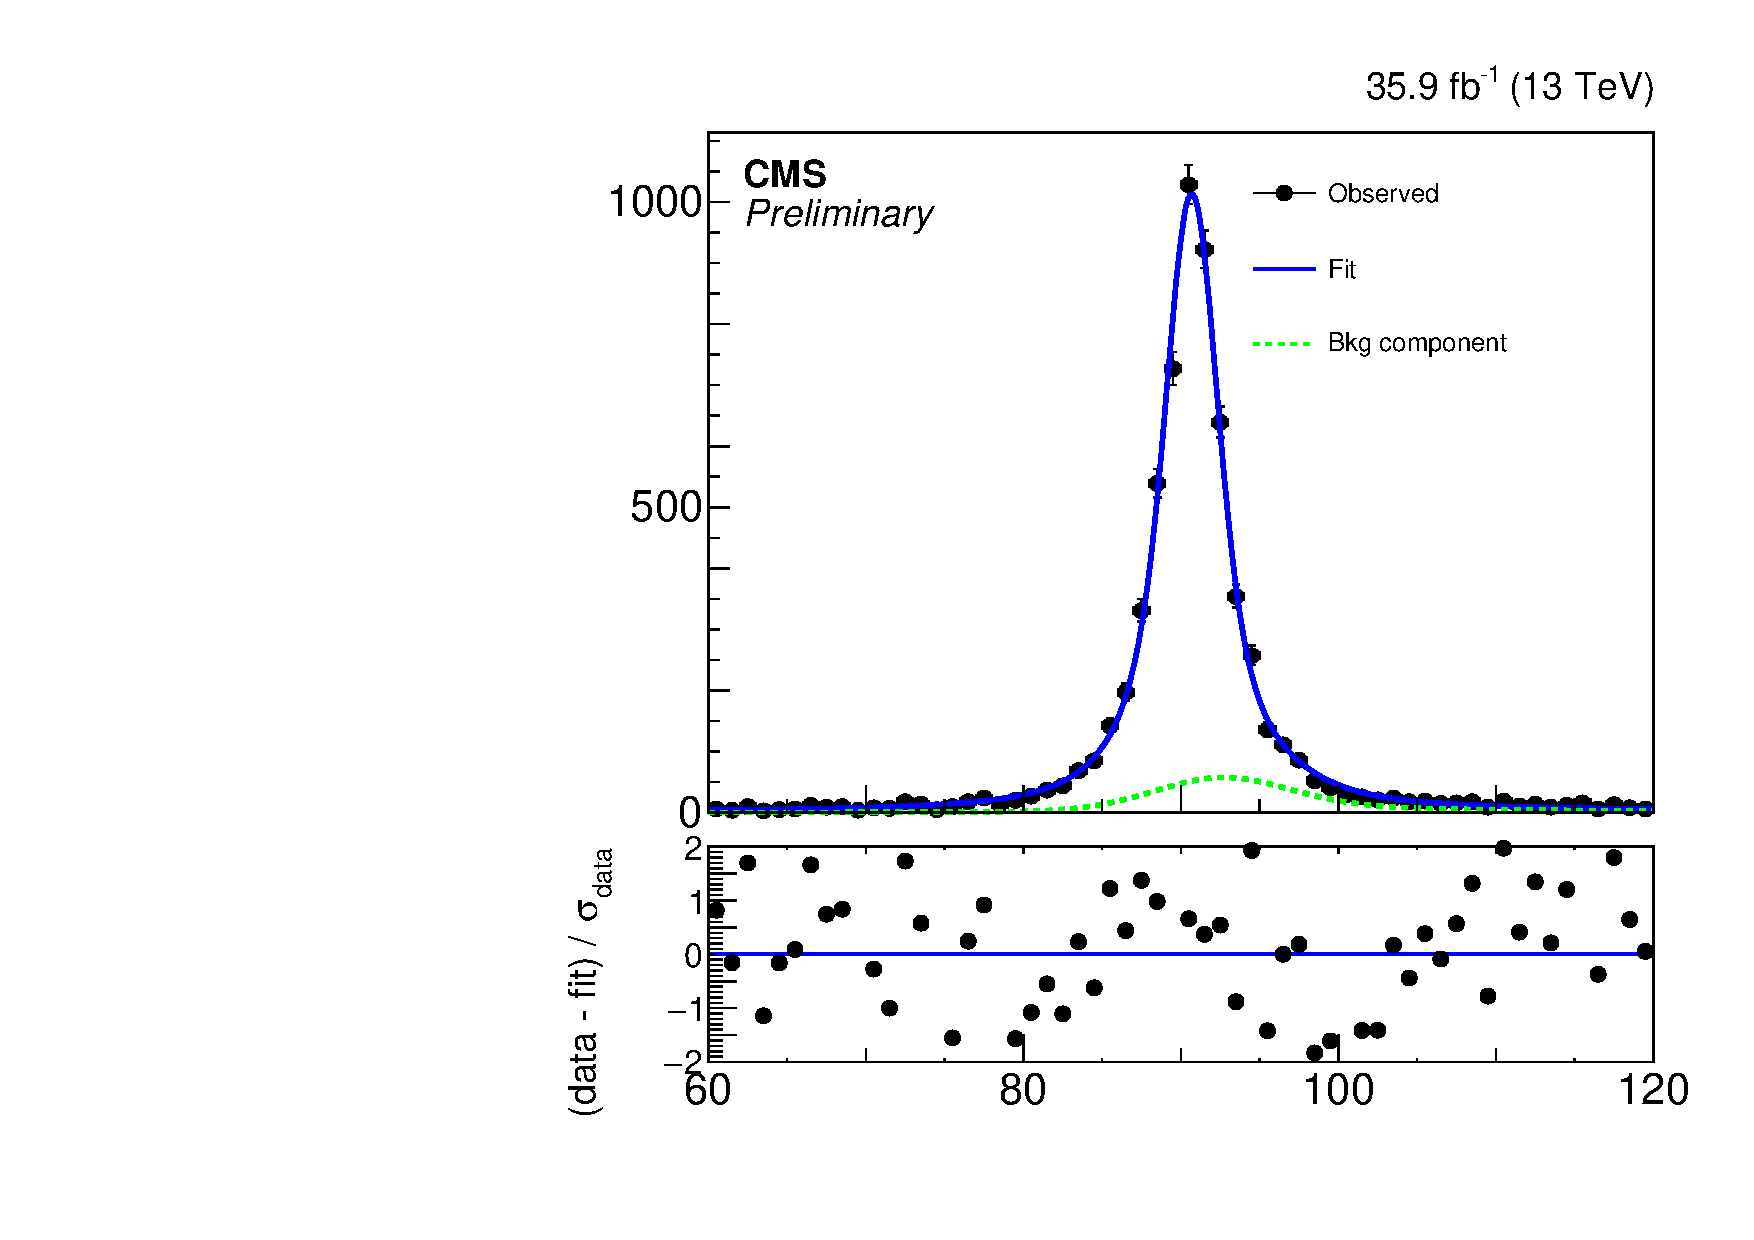
\includegraphics[width=0.47\textwidth]{Analysis/Figures/fit_data_ee_pt_200_250.pdf}
    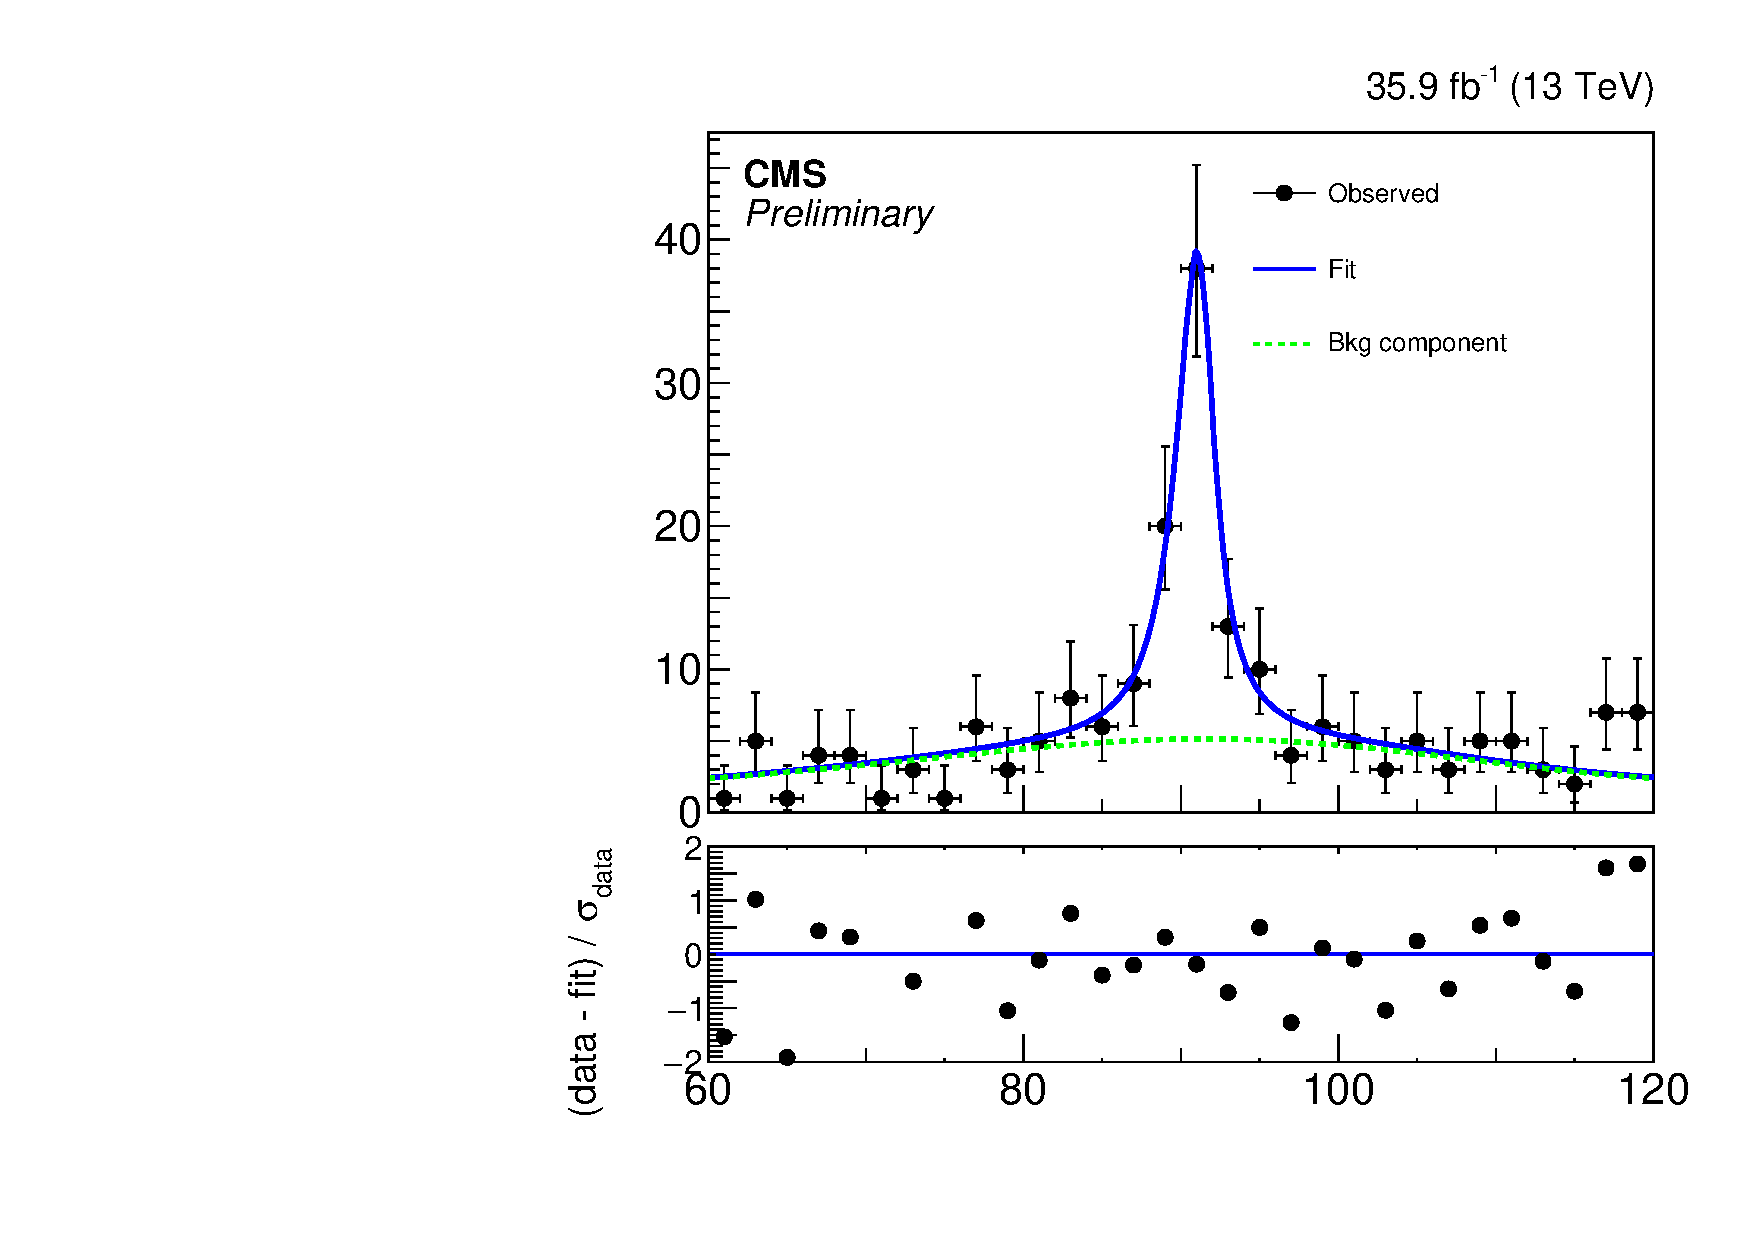
\includegraphics[width=0.47\textwidth]{Analysis/Figures/fit_data_eg_pt_200_250.pdf}
    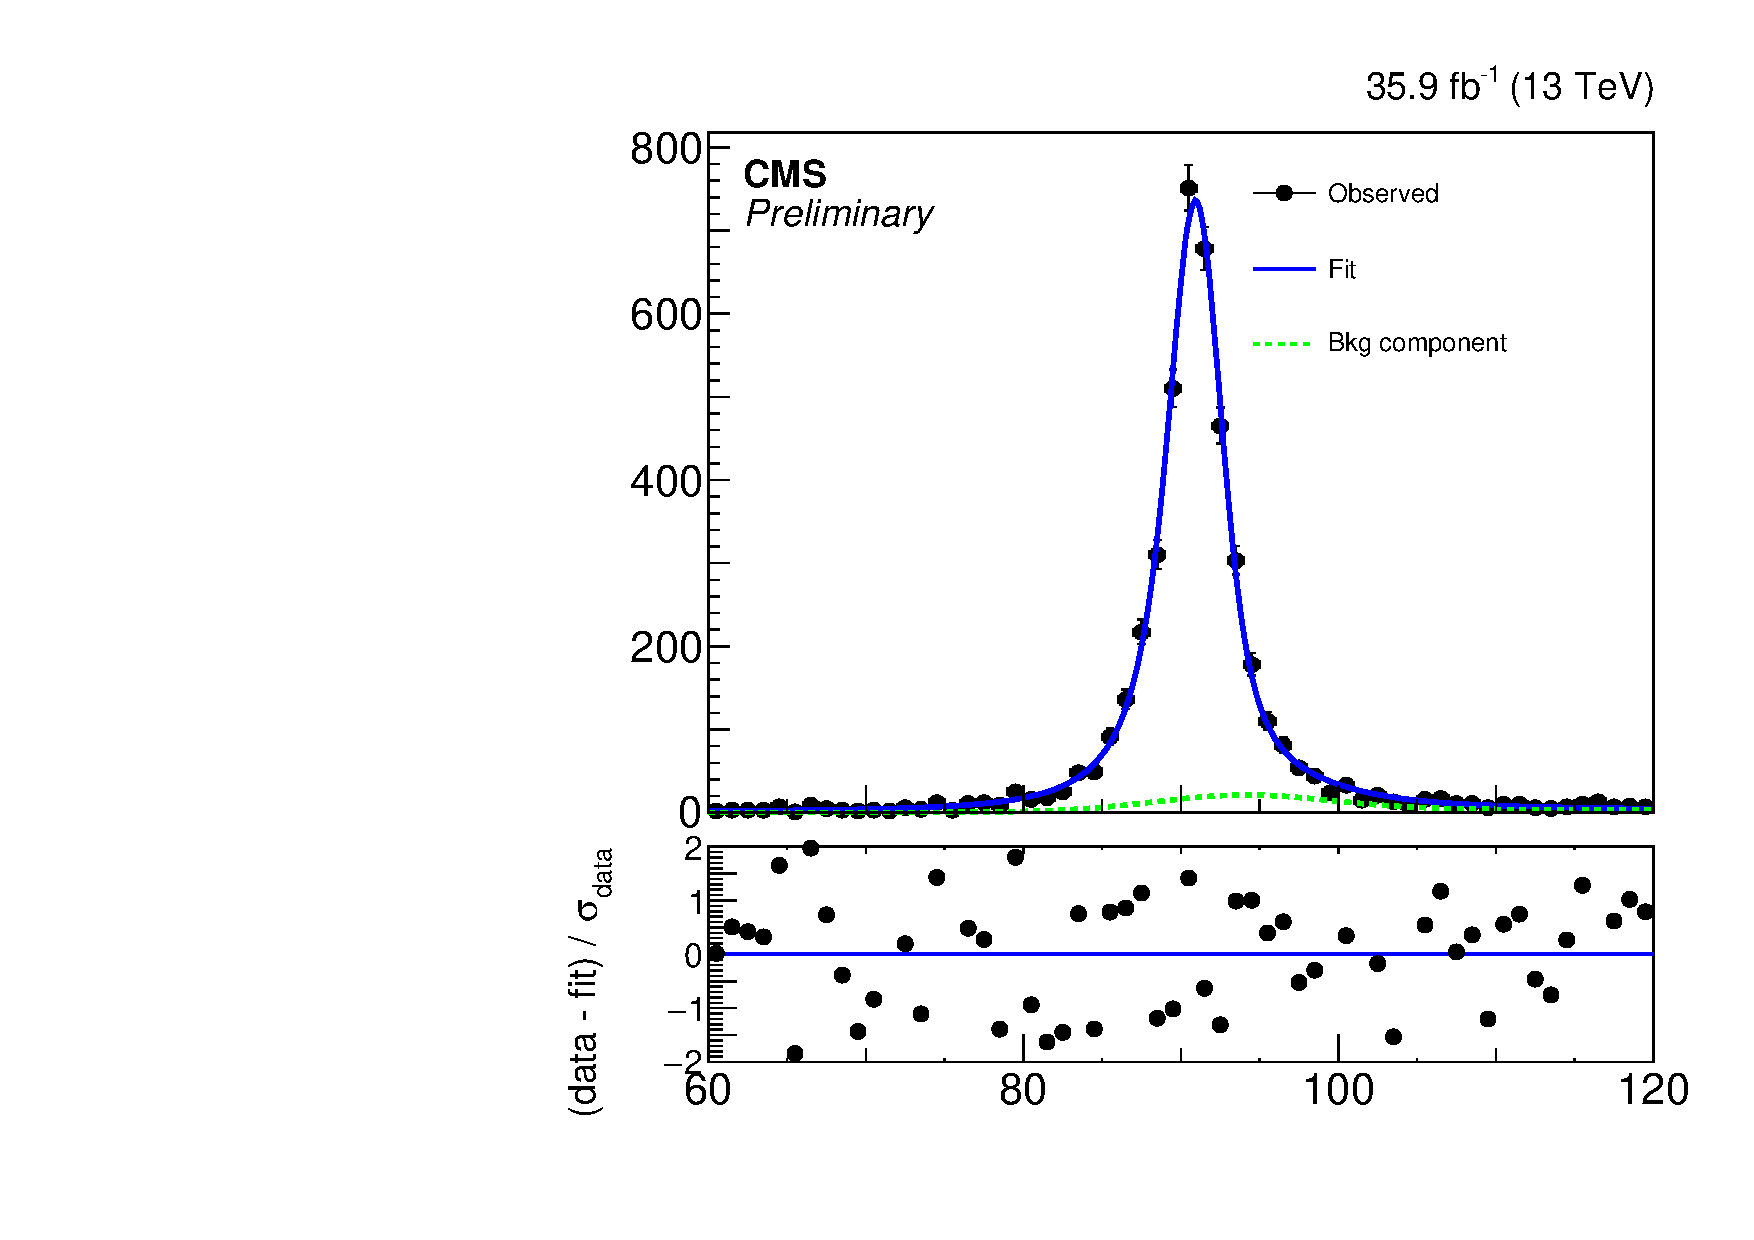
\includegraphics[width=0.47\textwidth]{Analysis/Figures/fit_data_ee_pt_250_6500.pdf}
    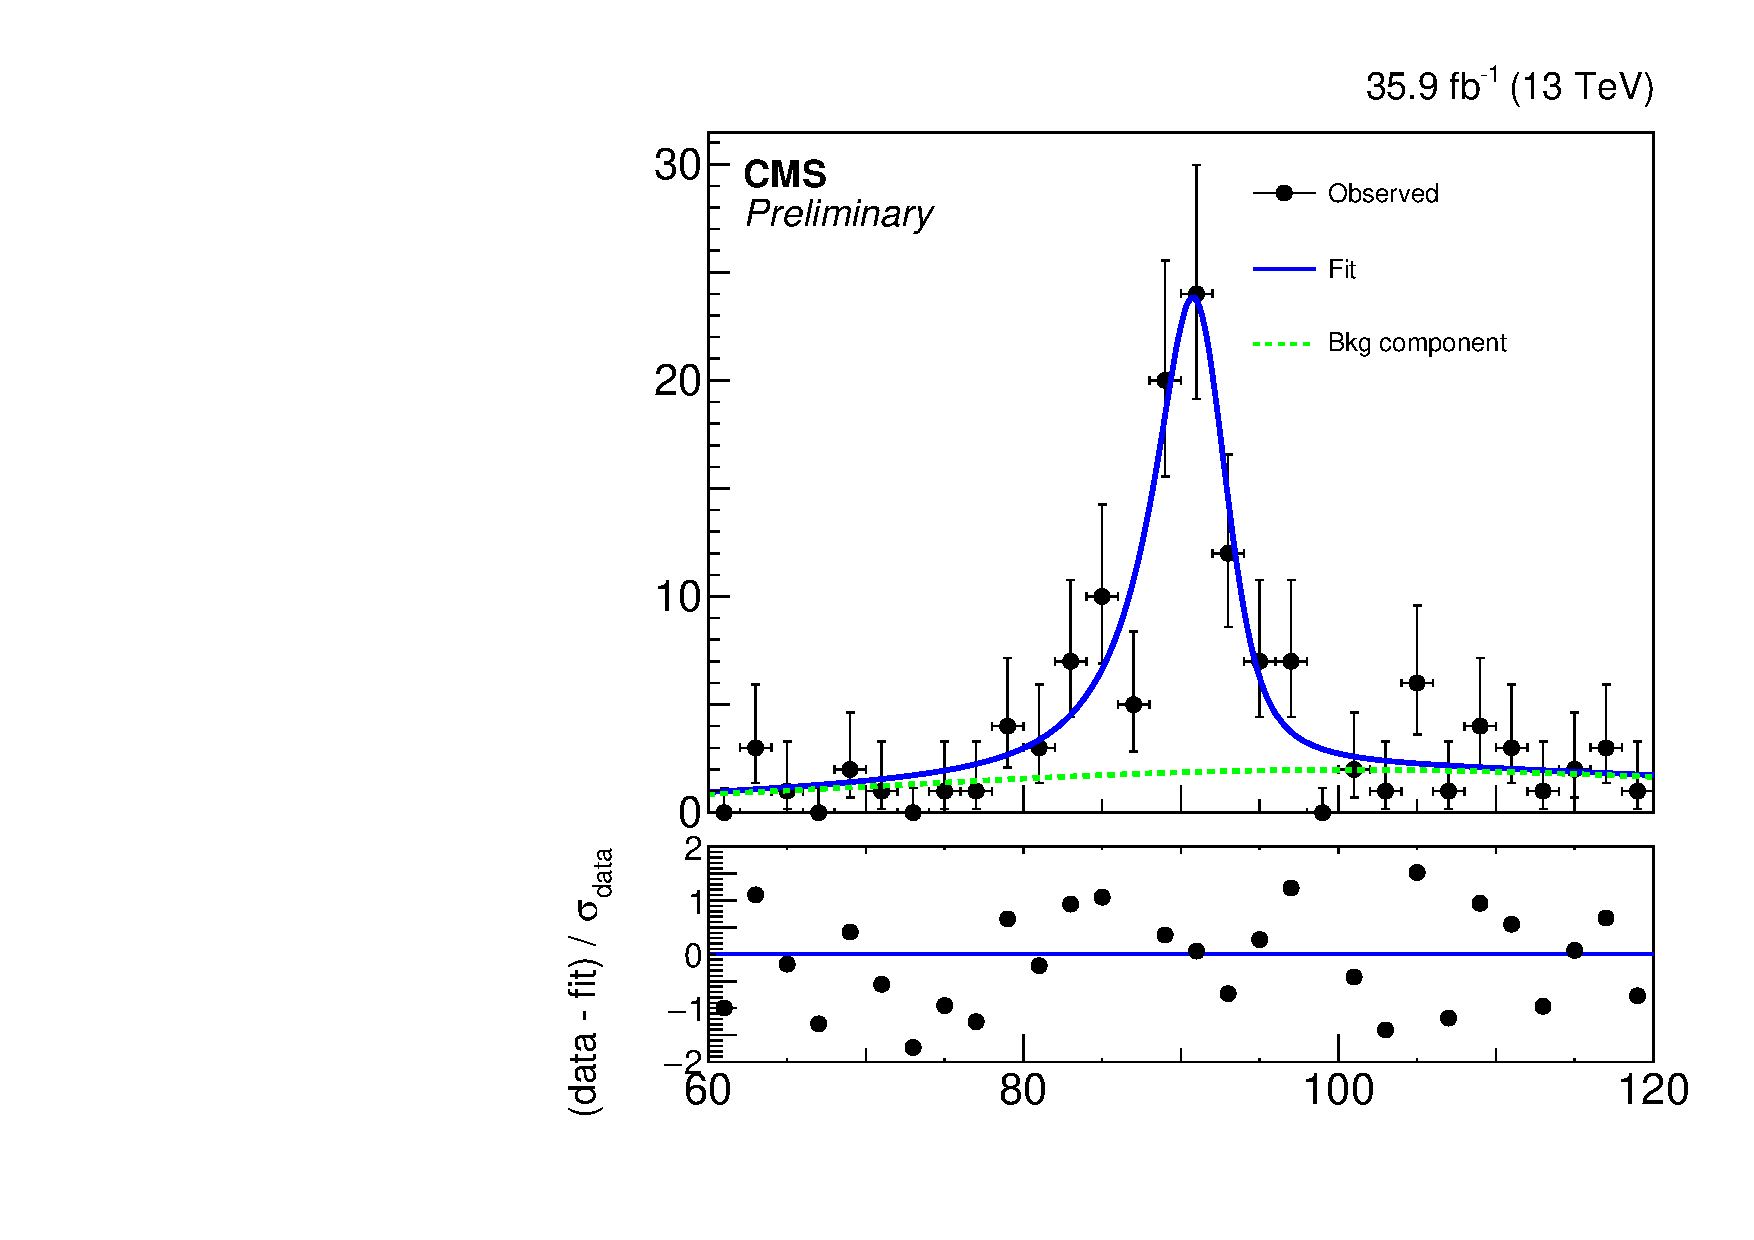
\includegraphics[width=0.47\textwidth]{Analysis/Figures/fit_data_eg_pt_250_6500.pdf}
    \caption{
      Fits to the mass distributions for \Pe\Pe\ (left) and \Pe\Pgg\ (right) selections, in bins of probe $\pt$: $175 < \pt < 200\GeV$ (top), $200 < \pt < 250\GeV$ (middle), $\pt > 250\GeV$ (bottom). 
      The blue solid line represents the full fit model, and the green dashed line its background component.
    }
    \label{fig:efake_fits}
  \end{center}
\end{figure}

Figure~\ref{fig:efake_fits} shows the six fits performed on \Pe\Pe\ and \Pe\Pgg\ in bins of probe $\pt$, from which the $R_{\Pe}$ factor used for the estimation of the electron misidentification background is derived.
Figure~\ref{fig:efake_frate} shows the derived $R_{\Pe}$ factor as a function of \ETg. 
The electron proxy sample is reweighted by $R_{\Pe}$ depending on the \pt\ of the electron object.

%%% this file has charged PF veto included, need to swap out
\begin{figure}[htbp]
  \begin{center}
    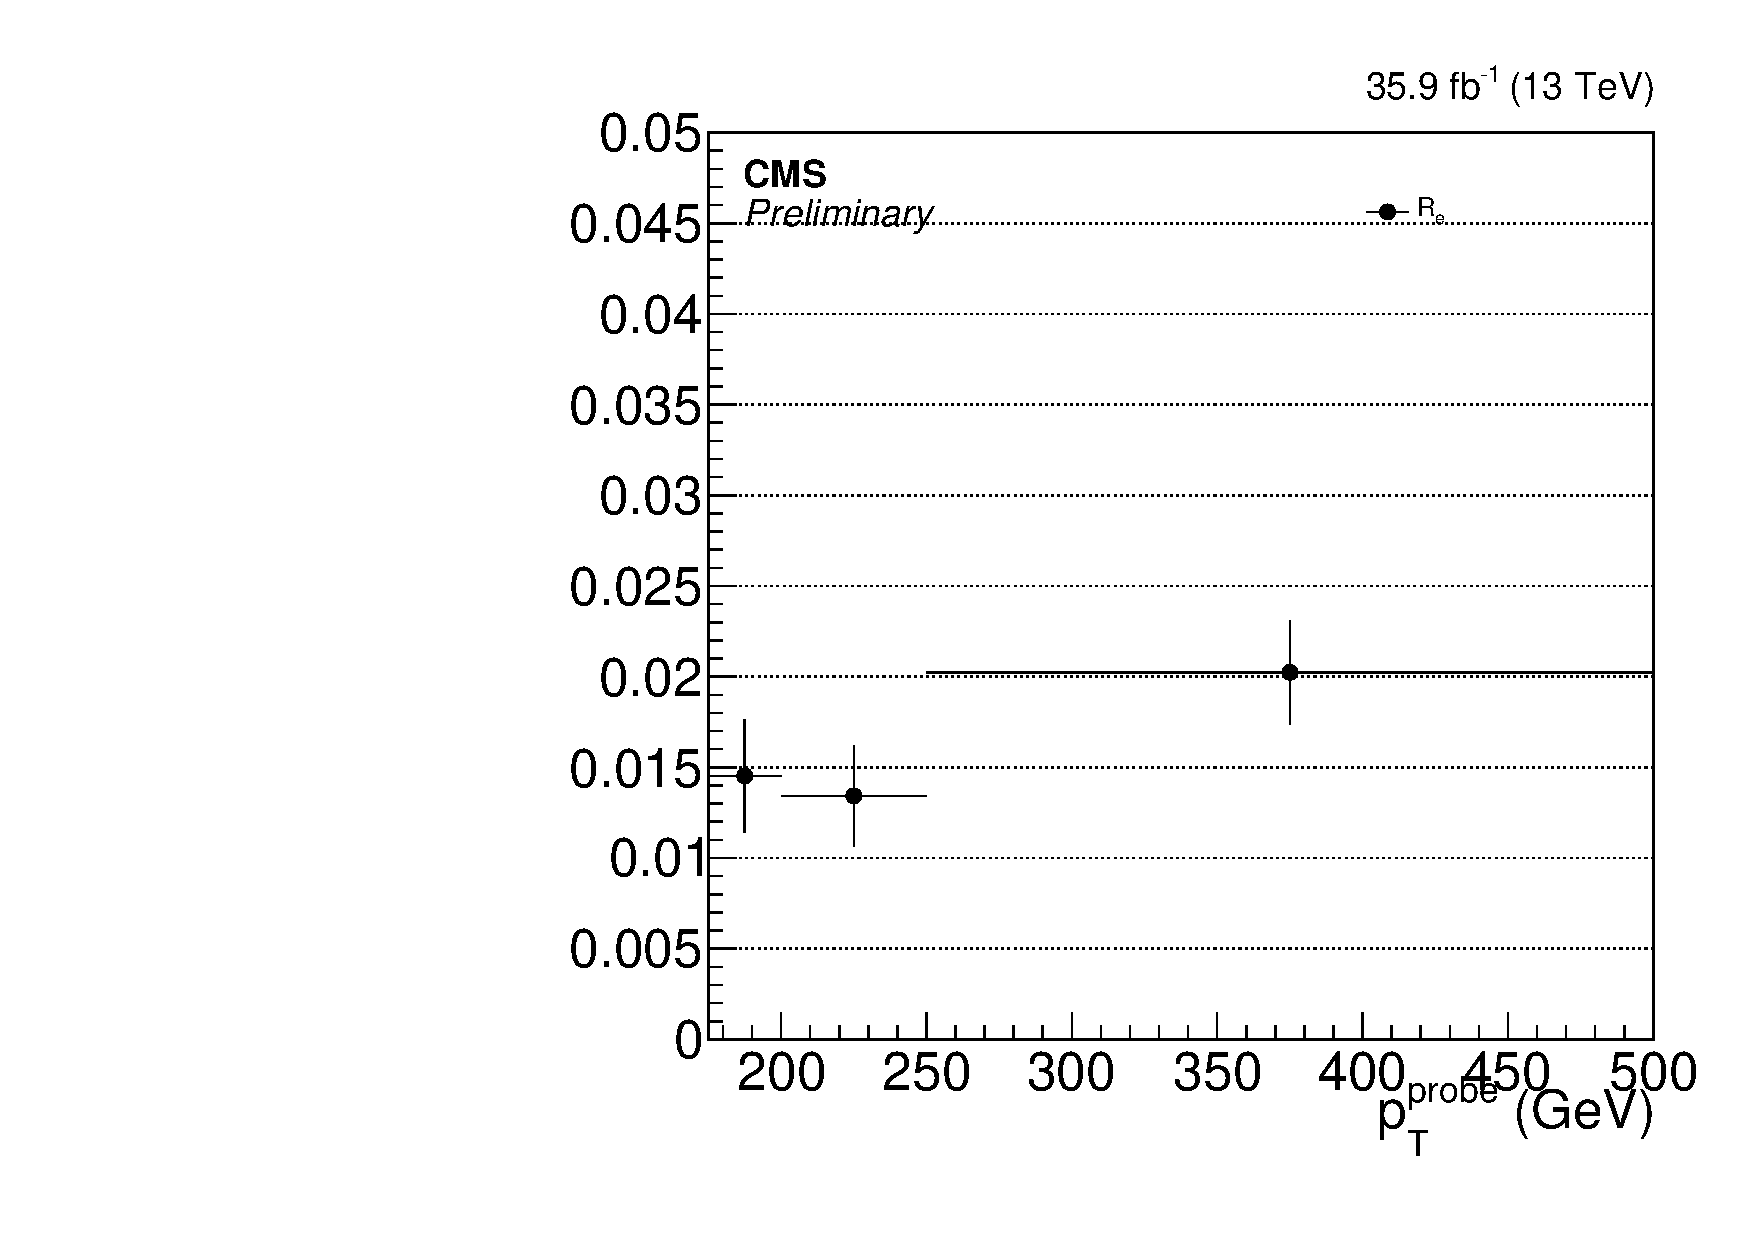
\includegraphics[width=0.49\textwidth]{Analysis/Figures/frate_data_ptalt.pdf} 
    \caption{
      Electron to photon fake rate $R_{\Pe}$.
    }
    \label{fig:efake_frate}
  \end{center}
\end{figure}
